% ─── Chapter 6: Digital Twin ─────────────────────────────────────────────────

% Slide: Client-Side Architecture (from thesis Ch.6)
\begin{frame}{Client-Side Software Architecture}
  \small
  \begin{columns}[T]
    \begin{column}{0.52\textwidth}
      The Digital Twin is a \textbf{purely client-side web application} (no server-side backend).
      \vspace{0.05cm}
      \begin{block}{Model-View-Controller (MVC)}
        \footnotesize
        \begin{itemize}
          \setlength{\itemsep}{1pt}
          \item \textbf{Model}: IGA-ROM engine executing hyper-reduced ECSW solver loops using \texttt{Float64Array} arrays.
          \item \textbf{View}: HTML5 Canvas rendering structural deformation and Von Mises stress heatmaps.
          \item \textbf{Controller}: Event listeners mapping UI parameter sliders directly to the ROM solver.
        \end{itemize}
      \end{block}
      \vspace{0.05cm}
      ROM datasets ($\boldsymbol{\Phi}$, $w_e$) serialized as compact \texttt{JSON} payloads.
    \end{column}
    \begin{column}{0.45\textwidth}
      \centering
      \begin{tikzpicture}[
        node distance=0.45cm,
        box/.style={rectangle, draw=cnamred, fill=cnamlightbg, thick, rounded corners,
                    minimum width=3.8cm, minimum height=0.7cm, align=center, font=\scriptsize}
      ]
        \node[box] (m) {\textbf{Model} — IGA-ROM Core\\{\footnotesize ECSW: $2.2$ ms/step}};
        \node[box, below=of m] (c) {\textbf{Controller} — User Sliders\\{\footnotesize $\mu$, $r$, $\sigma$ parameter inputs}};
        \node[box, below=of c] (v) {\textbf{View} — HTML5 Canvas\\{\footnotesize Von Mises heatmap @ 20 FPS}};
        \draw[<->, thick, cnamred] (m) -- (c);
        \draw[<->, thick, cnamred] (c) -- (v);
        \node[above=0.25cm of m, font=\tiny, align=center, draw=gray!50, rounded corners, fill=gray!10, inner sep=3pt] {JSON payloads loaded async};
      \end{tikzpicture}
    \end{column}
  \end{columns}
\end{frame}

% Slide: Reference Pullback Mapping Visualized
\begin{frame}{Reference Pullback Mapping Visualized}
  \centering
  \scalebox{0.8}{
  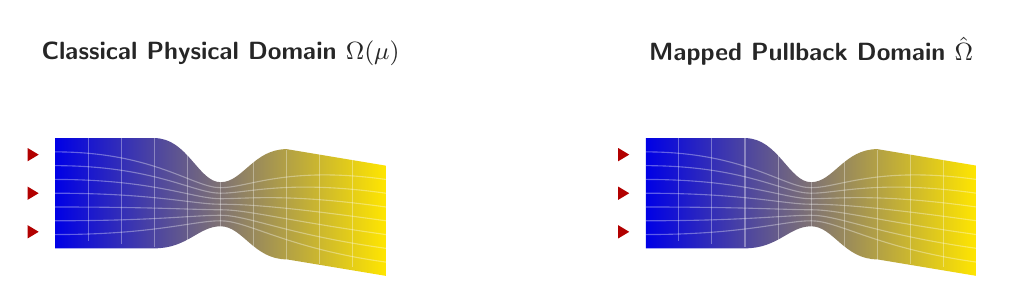
\begin{tikzpicture}[scale=1.0, >=stealth]
      % --- LEFT VIEWPORT: DEFORMED PHYSICAL DOMAIN ---
      \begin{scope}[xshift=-3.75cm, yshift=0cm, scale=0.7]
          \node[above=0.8cm, font=\small\bfseries\sffamily, text=black!85] at (0, 1.0) {Classical Physical Domain $\Omega(\boldsymbol{\mu})$};
          
          % Boundary conditions (clamped support triangles on left)
          \foreach \y in {-0.7, 0, 0.7} {
              \fill[red!70!black] (-3.3, \y) -- (-3.5, \y+0.12) -- (-3.5, \y-0.12) -- cycle;
          }
          
          % Deflected notched beam
          \shade[left color=blue!90!black, middle color=cyan!80, right color=yellow!80!orange] 
          (-3, -1) -- (-1.2, -1) 
          .. controls (-0.6, -1.0) and (-0.4, -0.6) .. (0, -0.6)
          .. controls (0.4, -0.6) and (0.6, -1.2) .. (1.2, -1.2)
          -- (3, -1.5) -- (3, 0.5) -- (1.2, 0.8)
          .. controls (0.6, 0.8) and (0.4, 0.2) .. (0, 0.2)
          .. controls (-0.4, 0.2) and (-0.6, 1.0) .. (-1.2, 1.0)
          -- (-3, 1) -- cycle;
          
          % Isoparametric mesh lines (curved to show deformation and parameterization)
          \foreach \y in {-0.75, -0.5, -0.25, 0, 0.25, 0.5, 0.75} {
              \draw[white, opacity=0.35, thin] (-3, \y)
              .. controls (-1.2, \y) and (-0.5, \y*0.4 - 0.2) .. (0, \y*0.4 - 0.2)
              .. controls (0.5, \y*0.4 - 0.2) and (1.2, \y - 0.25) .. (3, \y - 0.5);
          }
          \foreach \x in {-2.4, -1.8, -1.2, -0.6, 0, 0.6, 1.2, 1.8, 2.4} {
              \draw[white, opacity=0.35, thin] (\x, -1.1 - 0.1*\x) -- (\x, 0.9 - 0.1*\x);
          }
      \end{scope}
      
      % --- RIGHT VIEWPORT: STATIC REFERENCE PULLBACK ---
      \begin{scope}[xshift=3.75cm, yshift=0cm, scale=0.7]
          \node[above=0.8cm, font=\small\bfseries\sffamily, text=black!85] at (0, 1.0) {Mapped Pullback Domain $\hat{\Omega}$};
          
          % Boundary conditions (clamped support triangles on left)
          \foreach \y in {-0.7, 0, 0.7} {
              \fill[red!70!black] (-3.3, \y) -- (-3.5, \y+0.12) -- (-3.5, \y-0.12) -- cycle;
          }
          
          % Deflected notched beam (same as left)
          \shade[left color=blue!90!black, middle color=cyan!80, right color=yellow!80!orange] 
          (-3, -1) -- (-1.2, -1) 
          .. controls (-0.6, -1.0) and (-0.4, -0.6) .. (0, -0.6)
          .. controls (0.4, -0.6) and (0.6, -1.2) .. (1.2, -1.2)
          -- (3, -1.5) -- (3, 0.5) -- (1.2, 0.8)
          .. controls (0.6, 0.8) and (0.4, 0.2) .. (0, 0.2)
          .. controls (-0.4, 0.2) and (-0.6, 1.0) .. (-1.2, 1.0)
          -- (-3, 1) -- cycle;
          
          % Isoparametric mesh lines (same as left)
          \foreach \y in {-0.75, -0.5, -0.25, 0, 0.25, 0.5, 0.75} {
              \draw[white, opacity=0.35, thin] (-3, \y)
              .. controls (-1.2, \y) and (-0.5, \y*0.4 - 0.2) .. (0, \y*0.4 - 0.2)
              .. controls (0.5, \y*0.4 - 0.2) and (1.2, \y - 0.25) .. (3, \y - 0.5);
          }
          \foreach \x in {-2.4, -1.8, -1.2, -0.6, 0, 0.6, 1.2, 1.8, 2.4} {
              \draw[white, opacity=0.35, thin] (\x, -1.1 - 0.1*\x) -- (\x, 0.9 - 0.1*\x);
          }
      \end{scope}
  \end{tikzpicture}
  }
  \par\vspace{0.1cm}
  {\footnotesize Pulling the parameter-dependent physical domain $\Omega(\boldsymbol{\mu})$ back to a single reference coordinates space $\hat{\Omega}$ keeps the mesh nodes and basis functions static.}
\end{frame}

% Slide: Reference Config Mapping & Performance (from thesis Ch.6)
\begin{frame}{Reference Configuration Mapping — Performance}
  \small
  \begin{columns}[T]
    \begin{column}{0.54\textwidth}
      \begin{block}{FOM Pullback to Static $\hat{\Omega}$}
        \footnotesize
        \vspace{-0.15cm}
        \[
          \nabla_{\vect{x}}R_i = \mat{J}^{-T}(\boldsymbol{\xi};\boldsymbol{\mu})\,\nabla_{\boldsymbol{\xi}}\hat{R}_i
        \]
        \vspace{-0.3cm}
        \[
          K_{ij}(\boldsymbol{\mu}) = \int_{\hat{\Omega}} (\mat{J}^{-T}\nabla_{\boldsymbol{\xi}}\hat{R}_i):\mat{D}:(\mat{J}^{-T}\nabla_{\boldsymbol{\xi}}\hat{R}_j)\det(\mat{J})\,d\hat{\Omega}
        \]
        \vspace{-0.2cm}
      \end{block}
      \vspace{-0.05cm}
      \begin{exampleblock}{Key Advantages of Reference Mapping}
        \footnotesize
        \begin{itemize}
          \setlength{\itemsep}{1pt}
          \item Single mesh topology — no distortion or remeshing
          \item Static basis functions $\hat{R}_i$
          \item Offline precomputation of invariant terms
        \end{itemize}
      \end{exampleblock}
    \end{column}
    \begin{column}{0.42\textwidth}
      \begin{block}{Client-Side Benchmark}
        \centering\footnotesize
        \begin{tabular}{lcc}
          \toprule
          \textbf{Metric} & \textbf{Classical} & \textbf{Mapped} \\
          \midrule
          Assembly   & 35.10 ms & 0.90 ms \\
          ROM solver & 1.20 ms  & 0.40 ms \\
          Total/step & 36.30 ms & 1.30 ms \\
          Refresh    & 5 FPS    & 20 FPS  \\
          \midrule
          \textbf{Speedup} & Ref. & $\mathbf{38.4\times}$ \\
          \bottomrule
        \end{tabular}
      \end{block}
    \end{column}
  \end{columns}
\end{frame}

% Slide: Mapped vs. Non-Mapped ECSW
\begin{frame}{Mapped vs. Non-Mapped ECSW}
  \small
  The ECSW hyper-reduction algorithm integrates over a sparse active subset of elements $E^* \subset E$ with weights $w_e$:
  \[
    \mat{K}(\boldsymbol{\mu}) \approx \sum_{e \in E^*} w_e \mat{K}_e(\boldsymbol{\mu})
  \]
  \vspace{-0.15cm}
  \begin{columns}[T]
    \begin{column}{0.48\textwidth}
      \begin{alertblock}{Naive Non-Mapped Pipeline}
        \footnotesize
        If the physical mesh is regenerated (remeshed) for each shape change:
        \begin{itemize}
          \setlength{\itemsep}{1pt}
          \item Element volumes and node grids change continuously.
          \item The active subset $E^*$ and weights $w_e$ shift, requiring \textbf{re-training online}.
          \item Hyper-reduction speedup is lost.
        \end{itemize}
      \end{alertblock}
    \end{column}
    \begin{column}{0.48\textwidth}
      \begin{exampleblock}{Mapped Pullback Pipeline}
        \footnotesize
        By pulling back the equations of motion to reference configuration $\hat{\Omega}$:
        \begin{itemize}
          \setlength{\itemsep}{1pt}
          \item Reference mesh grid remains \textbf{strictly static} across all parameter states.
          \item A \textbf{single, fixed element set $E^*$} and weights $w_e$ is trained once offline.
          \item Enables real-time parameter sweeps.
        \end{itemize}
      \end{exampleblock}
    \end{column}
  \end{columns}
\end{frame}


